\documentclass[11pt]{article}

% Page formatting
\usepackage[a4paper, margin=2cm]{geometry}
\usepackage{setspace}
\usepackage{parskip}
\usepackage{microtype}
\usepackage{xcolor}
\usepackage{titlesec}
\usepackage{graphicx}
\usepackage{tikz}
\usetikzlibrary{arrows.meta, positioning, fit, backgrounds}
\newcommand{\code}[1]{\texttt{\detokenize{#1}}}
\usepackage{tabularx}
\usepackage{caption}
\newcolumntype{Y}{>{\raggedright\arraybackslash}X}
\captionsetup[table]{skip=6pt}
% Tables and lists
\usepackage{booktabs}
\usepackage{array}
\usepackage{float}
\usepackage{enumitem}

% Text formatting
\usepackage[T1]{fontenc}
\usepackage{lmodern}
\usepackage{hyperref}

\hypersetup{
    colorlinks=true,
    linkcolor=black,
    urlcolor=blue
}

\setstretch{1.03}
\setlist[itemize]{leftmargin=1.2em, itemsep=0.15em}

% Colours
\definecolor{bseblue}{RGB}{45,75,110}
\definecolor{lightgraytext}{RGB}{140,140,140}
\definecolor{zonegray}{RGB}{245,247,250}

% Section heading style
\titleformat{\section}
  {\normalfont\Large\bfseries\color{bseblue}}
  {}
  {0em}
  {}

\titleformat{\subsection}
  {\normalfont\large\bfseries\color{bseblue}}
  {}
  {0em}
  {}

\titlespacing*{\section}{0pt}{0.8em}{0.35em}
\titlespacing*{\subsection}{0pt}{0.55em}{0.2em}

\begin{document}

\begin{center}
    {\Large\bfseries\color{bseblue} Lab 3: Big Data Architectures \par}
    \vspace{0.1em}
    {\large 23D020 Big Data Management for Data Science \par}
    \vspace{0.1em}
    {\normalsize Anabel Pichardo, Cameron Armour \par}
    \vspace{0.1em}
    {\normalsize\color{lightgraytext} June 2026 \par}
\end{center}

\vspace{-0.5em}

\section*{A.1 Datasets and Analysis}

We predict the housing price tier of a Barcelona neighbourhood in a given year. The target has three classes, low, mid, and high, defined as the per-year terciles of the average sale price per square metre. The unit of analysis is the neighbourhood-year, identified by the official neighbourhood code \texttt{Codi\_Barri} and the year.

We integrate three Open Data BCN datasets, all at the neighbourhood-year grain:

\begin{table}[H]
\centering
\begin{tabularx}{0.95\textwidth}{@{} l c c Y c @{}}
\toprule
\textbf{Dataset} & \textbf{Format} & \textbf{Coverage} & \textbf{Provides} & \textbf{Role} \tabularnewline
\midrule
Family disposable income (RFD) & CSV & 2007--2017 & Income index & Feature \tabularnewline
Population and density & JSON & 2010--2021 & Population, density, surface & Feature \tabularnewline
Housing sale price & JSON & 2013--2017 & Sale price per m$^2$ & Target source \tabularnewline
\bottomrule
\end{tabularx}
\caption{Selected Datasets}
\end{table}
\vspace{-0.5em}
All three carry \texttt{Codi\_Barri} and a year, so they join exactly and need no name reconciliation. Their common period is 2013 to 2017. An inner join on neighbourhood and year over this window yields 359 rows with no missing values in the retained columns. The features are the income index, population, gross density, net density, surface, and a per-year rank of the income index. The price columns define the label, so we remove them from the features to avoid leakage.

We predict the price tier rather than an income or density tier for two reasons. With income as the label, the density data alone already separates the classes well and the price data adds no value, so the third dataset would not be justified. With density as the label, the anti-leakage rule forces us to drop population and surface as well, since the density measures are built from them, which leaves almost no usable features. Predicting the price tier keeps both income and density as informative, non-leaking predictors. Cutting the tiers per year removes the city-wide price increase across 2013 to 2017, so the label reflects a neighbourhood's standing relative to the city in that year. The resulting classes are balanced, with 119, 120, and 120 members.

We also reviewed the unemployment, incidence, and real-estate listing datasets and did not use them. The unemployment and incidence files are truncated samples, returning about one hundred records per year and, for unemployment, a single month, with the 2015 unemployment file empty, which leaves too little signal at the neighbourhood-year grain. The listing dataset covers only 2020 and 2021, so it does not overlap the income and price series.
\section*{A.2 Architecture}

The architecture is organised as a set of Spark DataFrame pipelines over three data lake zones, followed by a Spark ML and MLflow modelling pipeline. We separate these stages because each zone has a different responsibility. The Landing Zone preserves a reproducible raw snapshot, the Formatted Zone applies reusable cleaning and typing rules, and the Exploitation Zone is specific to predicting Barcelona neighbourhood price tiers. The Formatted and Exploitation zones are partitioned by year because downstream joins and model training operate over the shared 2013--2017 window.

\begin{figure}[H]
\centering
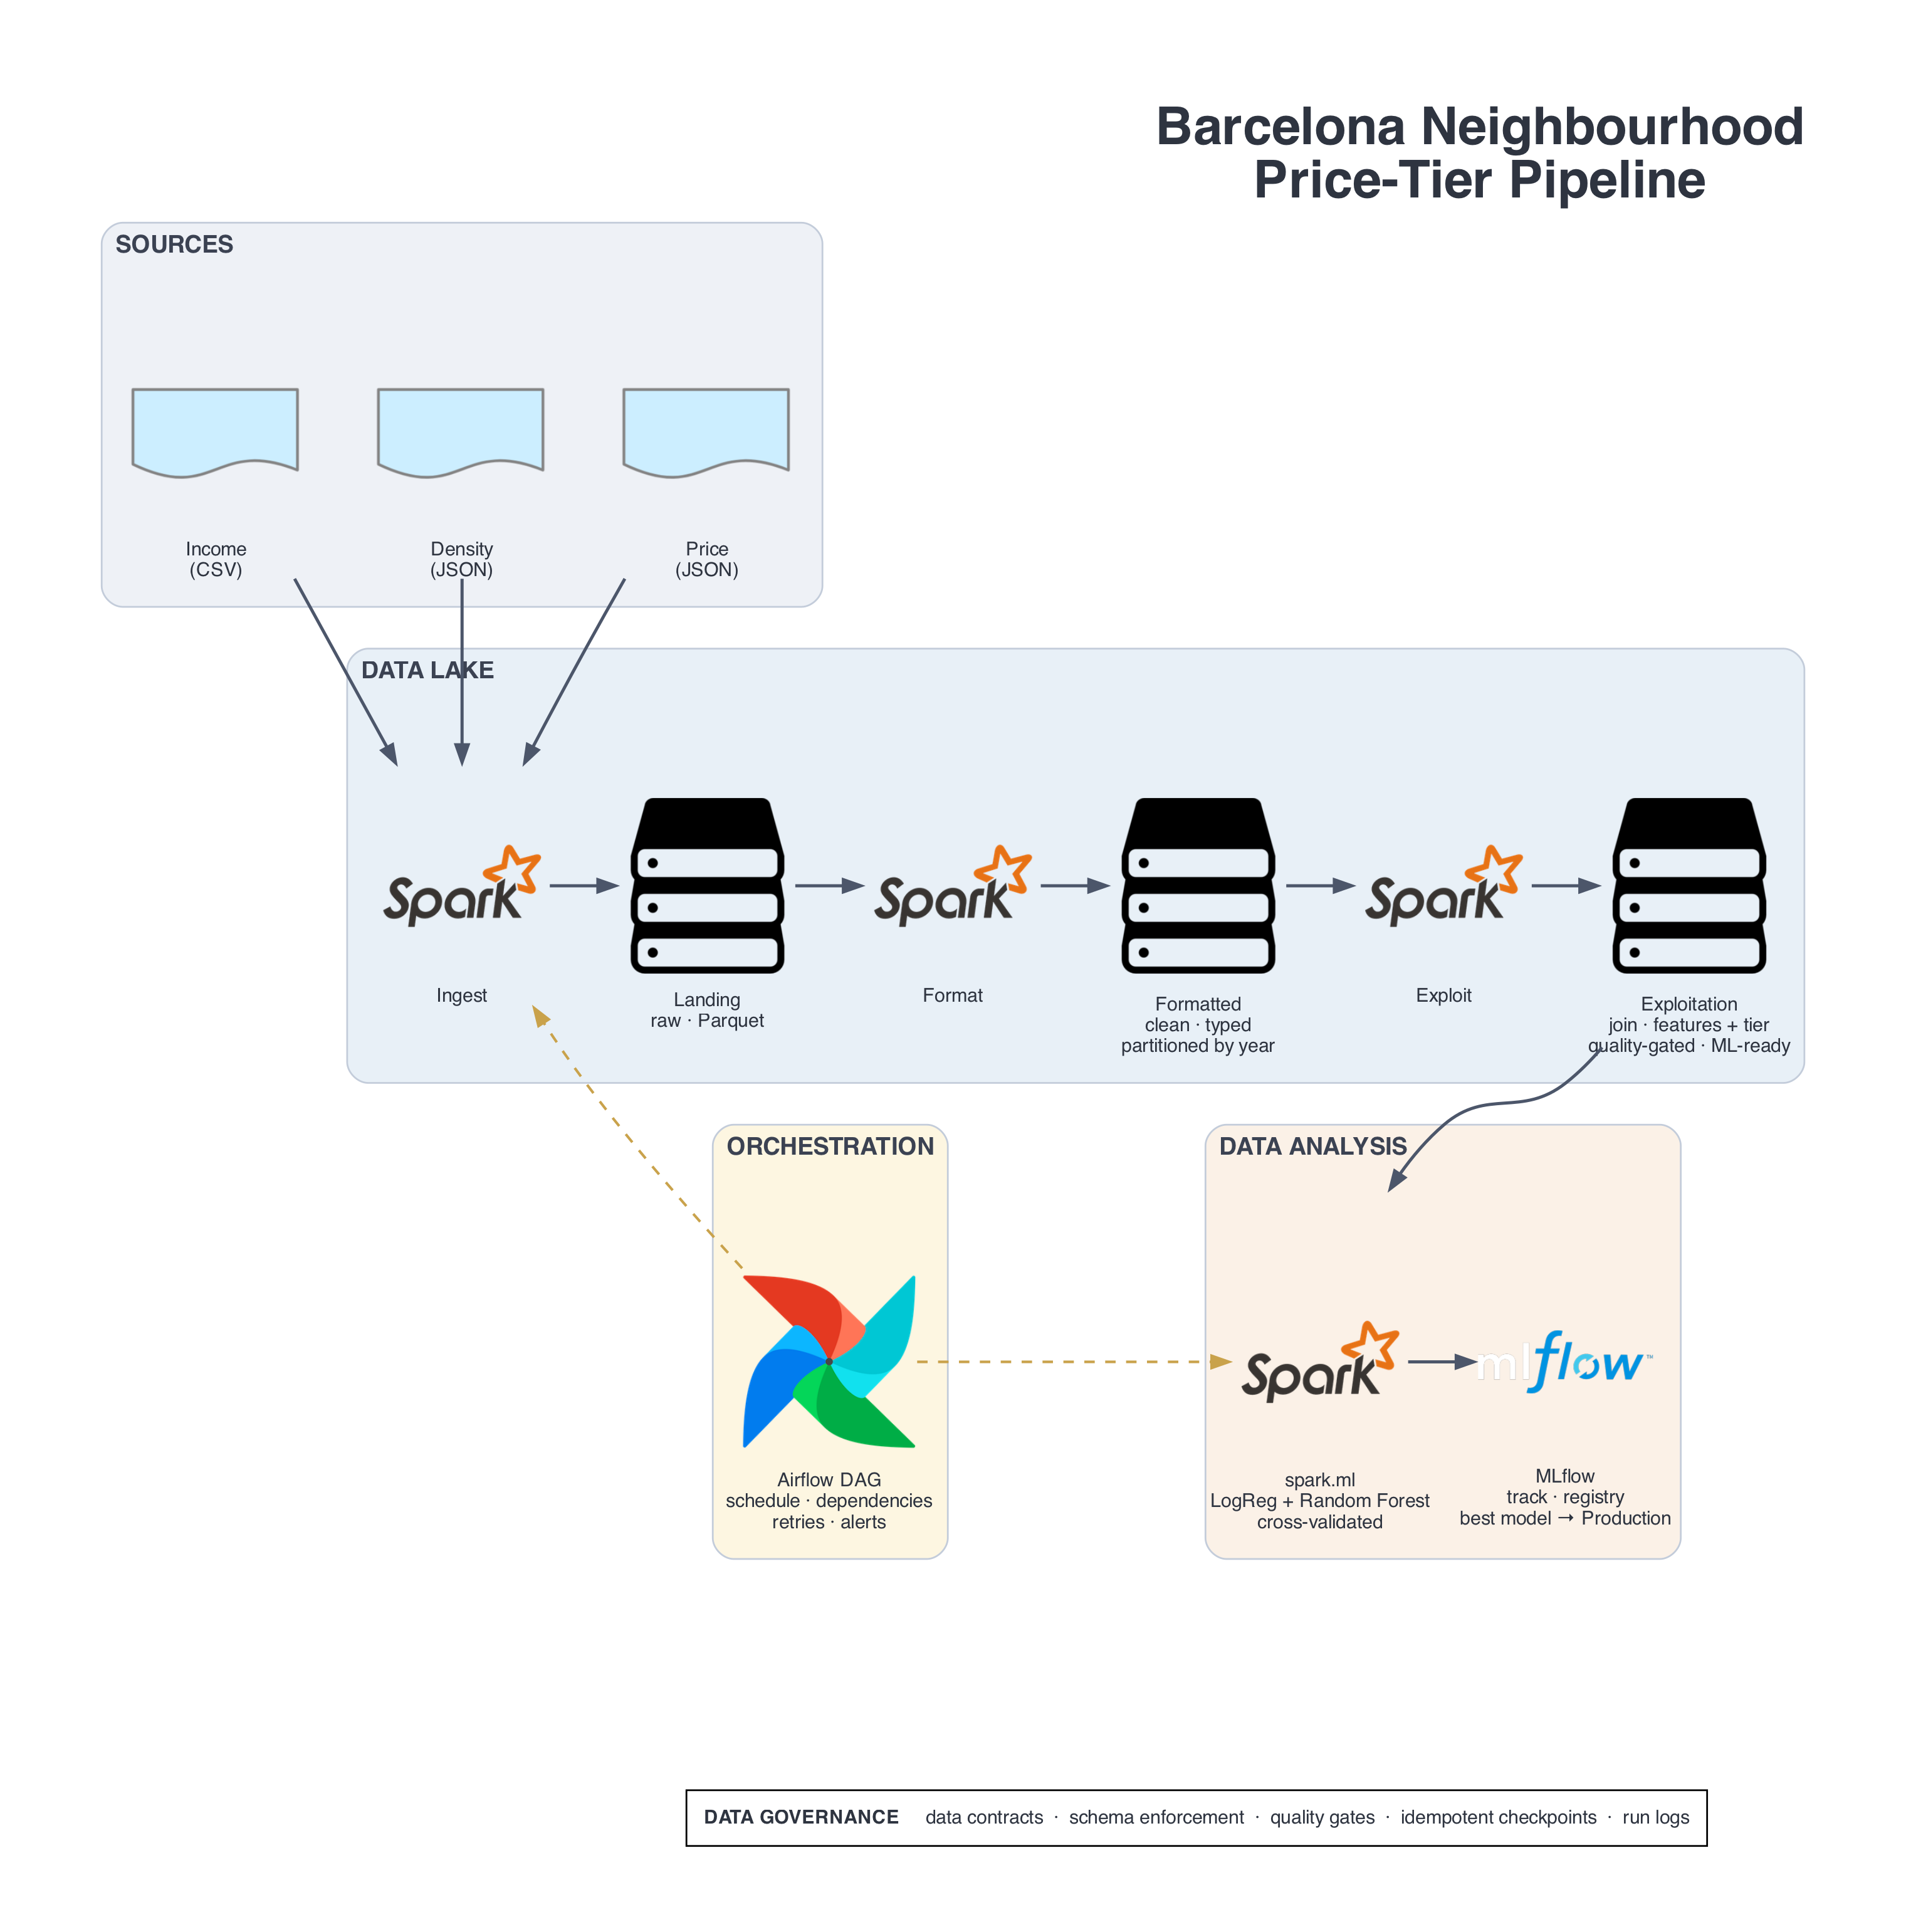
\includegraphics[width=0.75\textwidth]{pipeline_architecture.png}
\caption{High-level architecture of the Barcelona neighbourhood price-tier pipeline.}
\end{figure}

Figure 1 shows the complete flow from source files to model management. The important design decision is that modelling does not read directly from the raw or formatted data. Instead, it consumes one explicit exploitation table, built at the neighbourhood-year grain. This keeps the machine-learning input stable and makes it clear where features and labels are created.

Figure 2 expands the Spark pipelines and groups related Spark operations into boxes.

\begin{figure}[H]
\centering
\resizebox{\textwidth}{!}{
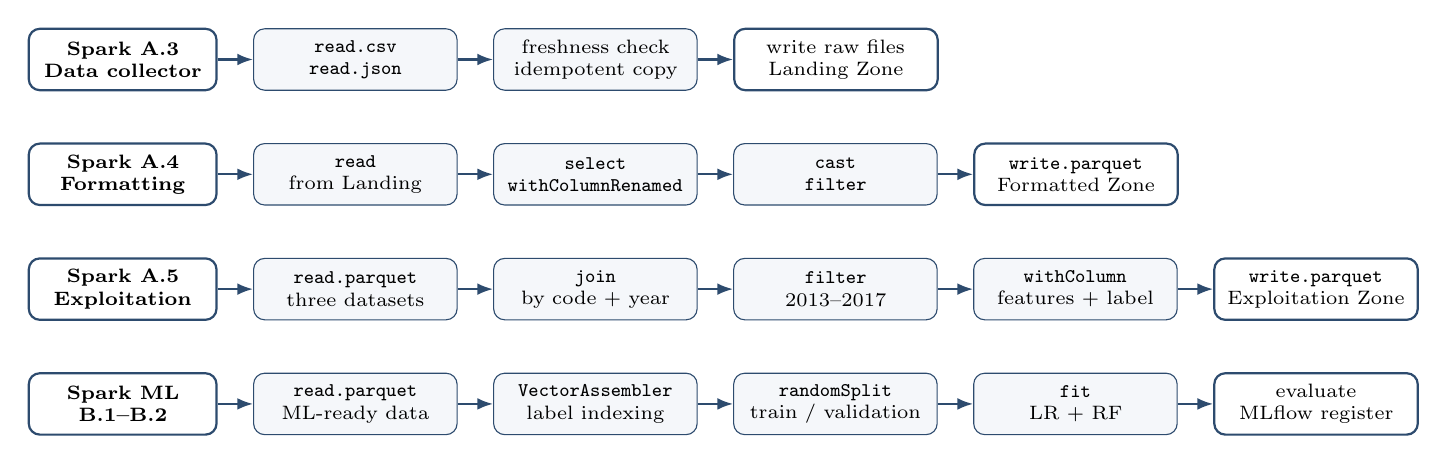
\begin{tikzpicture}[
    node distance=0.45cm and 0.45cm,
    stage/.style={
        rectangle,
        rounded corners,
        draw=bseblue,
        thick,
        fill=white,
        align=center,
        text width=2.15cm,
        minimum height=0.78cm,
        font=\scriptsize\bfseries
    },
    op/.style={
        rectangle,
        rounded corners,
        draw=bseblue,
        fill=zonegray,
        align=center,
        text width=2.35cm,
        minimum height=0.78cm,
        font=\scriptsize
    },
    action/.style={
        rectangle,
        rounded corners,
        draw=bseblue,
        thick,
        fill=white,
        align=center,
        text width=2.35cm,
        minimum height=0.78cm,
        font=\scriptsize
    },
    arrow/.style={-{Latex[length=2mm]}, thick, color=bseblue}
]

% A3 row
\node[stage] (a3) {Spark A.3\\Data collector};
\node[op, right=of a3] (a3a) {\texttt{read.csv}\\\texttt{read.json}};
\node[op, right=of a3a] (a3b) {freshness check\\idempotent copy};
\node[action, right=of a3b] (a3c) {write raw files\\Landing Zone};
\draw[arrow] (a3) -- (a3a);
\draw[arrow] (a3a) -- (a3b);
\draw[arrow] (a3b) -- (a3c);

% A4 row
\node[stage, below=0.65cm of a3] (a4) {Spark A.4\\Formatting};
\node[op, right=of a4] (a4a) {\texttt{read}\\from Landing};
\node[op, right=of a4a] (a4b) {\texttt{select}\\\texttt{withColumnRenamed}};
\node[op, right=of a4b] (a4c) {\texttt{cast}\\\texttt{filter}};
\node[action, right=of a4c] (a4d) {\texttt{write.parquet}\\Formatted Zone};
\draw[arrow] (a4) -- (a4a);
\draw[arrow] (a4a) -- (a4b);
\draw[arrow] (a4b) -- (a4c);
\draw[arrow] (a4c) -- (a4d);

% A5 row
\node[stage, below=0.65cm of a4] (a5) {Spark A.5\\Exploitation};
\node[op, right=of a5] (a5a) {\texttt{read.parquet}\\three datasets};
\node[op, right=of a5a] (a5b) {\texttt{join}\\by code + year};
\node[op, right=of a5b] (a5c) {\texttt{filter}\\2013--2017};
\node[op, right=of a5c] (a5d) {\texttt{withColumn}\\features + label};
\node[action, right=of a5d] (a5e) {\texttt{write.parquet}\\Exploitation Zone};
\draw[arrow] (a5) -- (a5a);
\draw[arrow] (a5a) -- (a5b);
\draw[arrow] (a5b) -- (a5c);
\draw[arrow] (a5c) -- (a5d);
\draw[arrow] (a5d) -- (a5e);

% B row
\node[stage, below=0.65cm of a5] (b) {Spark ML\\B.1--B.2};
\node[op, right=of b] (ba) {\texttt{read.parquet}\\ML-ready data};
\node[op, right=of ba] (bb) {\texttt{VectorAssembler}\\label indexing};
\node[op, right=of bb] (bc) {\texttt{randomSplit}\\train / validation};
\node[op, right=of bc] (bd) {\texttt{fit}\\LR + RF};
\node[action, right=of bd] (be) {evaluate\\MLflow register};
\draw[arrow] (b) -- (ba);
\draw[arrow] (ba) -- (bb);
\draw[arrow] (bb) -- (bc);
\draw[arrow] (bc) -- (bd);
\draw[arrow] (bd) -- (be);

\end{tikzpicture}
}
\caption{Spark pipelines expressed as grouped PySpark DataFrame and Spark ML operations. Grey boxes are transformations; white final boxes are materialisation, evaluation, or registration steps.}
\end{figure}

The architecture separates deterministic data preparation from learned model training. The Exploitation Zone fixes the modelling grain, joins the standardised datasets, creates the target and removes leakage-prone price fields. The Spark ML stage then consumes this stable table to train, compare and register models. Airflow orchestrates these stages in dependency order, so each downstream task runs only after its required upstream outputs have been rebuilt. This gives the pipeline a single control layer for scheduling, parallel task execution, failure handling and reruns.

\section*{B.3 Model Training and Validation Results}

The final exploitation table contains 359 neighbourhood-year rows after joining the three formatted datasets over the shared 2013--2017 period. As mentioned above, the target is balanced by construction as price per square metre is converted into three within-year tiers. This makes accuracy meaningful, while weighted recall, weighted precision and F1 are also reported to check that performance is not driven by a single class.

The model input contains only non-price features: \code{rfd_index}, \code{population}, \code{density_gross}, \code{density_net}, and \code{surface}. The raw price variables used to create the target are dropped before training. The training job uses a fixed seed of 42 and an 80/20 train-validation split after sorting the exploitation table, making the validation results reproducible. Each algorithm is wrapped in a Spark ML pipeline consisting of a target \code{StringIndexer}, a \code{VectorAssembler}, and the classifier.

\begin{figure}[H]
\centering
\includegraphics[width=0.75\textwidth]{model_results.png}
\end{figure}

The validation results show that Random Forest performs consistently better than Logistic Regression across all reported metrics. Random Forest scores about 0.83 for accuracy, weighted recall, weighted precision and F1, while Logistic Regression is around 0.72. Since the target classes are balanced by construction, accuracy is a meaningful headline metric, but the similar improvements in precision, recall and F1 suggest that the Random Forest advantage is not limited to one class or one type of error.

This result suggests that the relationship between neighbourhood income, population, density, surface and price tier is not purely linear. Logistic Regression can only model linear class boundaries, whereas Random Forest can capture thresholds and interactions between variables, such as cases where income has a different relationship with price tier depending on density or neighbourhood size. However, the dataset is small, with 359 neighbourhood-year observations, so the results should still be interpreted cautiously.

MLflow is used for model management. Each run logs the model type, selected hyperparameters, feature list, validation metrics, per-class precision/recall and the fitted Spark pipeline artifact. The training job ranks runs by validation accuracy, registers the best model under \code{barcelona_price_tier}, promotes it to production, reloads the registered model, and evaluates it again. The reloaded model obtains the same validation accuracy of 0.83, confirming that the registered artifact can be recovered and used for prediction.

\section*{Assumptions and Justifications}
\textbf{Data grain and joining.} We use neighbourhood-year as the common grain because it is the most detailed level at which the selected income, density and price datasets can be aligned consistently. This avoids aggregating to district level, which would lose neighbourhood variation, while also avoiding a finer grain that some sources cannot support. We use an inner join over the shared 2013--2017 window so that every modelling row is complete and no imputation is needed. The trade-off is that the final table is smaller, but the retained rows are directly comparable across all three sources.

\textbf{A.3--A.5 Data engineering.} The zones are separated so that each stage has a clear responsibility. The Landing Zone stores refreshed source snapshots as Parquet with ingestion metadata and minimal schema projection, giving a reproducible copy of the inputs while avoiding early analysis-specific cleaning. Explicit Spark schemas are used instead of automatic inference because several fields, such as the income index and price values, need consistent types across runs. 

\textbf{Leakage and validation checks.} Price fields are needed to construct \code{price_tier}, but they are removed from the feature matrix before training so that the model cannot directly recover the answer from the target source. This matters because otherwise the validation accuracy would overstate the model's real predictive value. The exploitation contract checks that the final table is non-empty, has the expected columns, contains no nulls in key features or labels, has unique \code{(Codi_Barri, year)} rows and includes all three target classes. These checks do not prove that the model is optimal, but they reduce the risk of training on a broken or inconsistent dataset.

\textbf{B.1--B.2 Modelling.} We use a fixed seed so that the train-validation split and model comparison are reproducible. The 80/20 split keeps most observations for training while reserving a held-out validation set for comparison. Three-fold cross-validation is applied on the training set to tune hyperparameters without using the validation set directly. This is appropriate for a small lab dataset, but the random split may still be optimistic because neighbouring years for the same area can appear in both train and validation. MLflow records parameters, metrics, feature lists and fitted Spark models, and the best run is registered as the production model so that the chosen model can be reloaded without hardcoding a run-specific path.

\textbf{C.1--C.2 Orchestration.} The Airflow DAG runs daily at midnight with \code{catchup=False}. Daily scheduling is a conservative choice for the lab reflecting our lack of detailed knowledge of the source update frequency. If the real update timing was known, the schedule could be changed to match it more closely. The DAG starts with a preflight check, then runs ingestion, formatting, exploitation and modelling in dependency order so that downstream stages only run after their inputs have been rebuilt. Each task has two retries, a five-minute retry delay and a 30-minute timeout to handle transient failures. Failure and completion alerts are implemented through Airflow callbacks that emit explicit alert messages in the task logs. We initially implemented email alerts (and left evidence of this in the scripts), but removed these to avoid requiring configuration for marking. In a production deployment, the same callbacks could be connected to email or another external notification service.

\textbf{Limitations.} The joined dataset is small because the common period is limited by the price series, so the validation metrics should be interpreted cautiously. The model predicts relative price tier rather than exact price per square metre, which fits the classification task and removes the city-wide price trend, but it also loses within-tier variation. Future work could add newer socioeconomic data, extend the feature set with other neighbourhood-level variables, and use time-based validation by training on earlier years and validating on later years.


\end{document}
